\begin{scanpage}{0067}{50}
\begingroup\setlength{\abovedisplayskip}{4pt}\setlength{\belowdisplayskip}{4pt}\setlength{\parskip}{3pt}
\begin{minipage}[t]{.43\linewidth}\vspace{0pt}\centering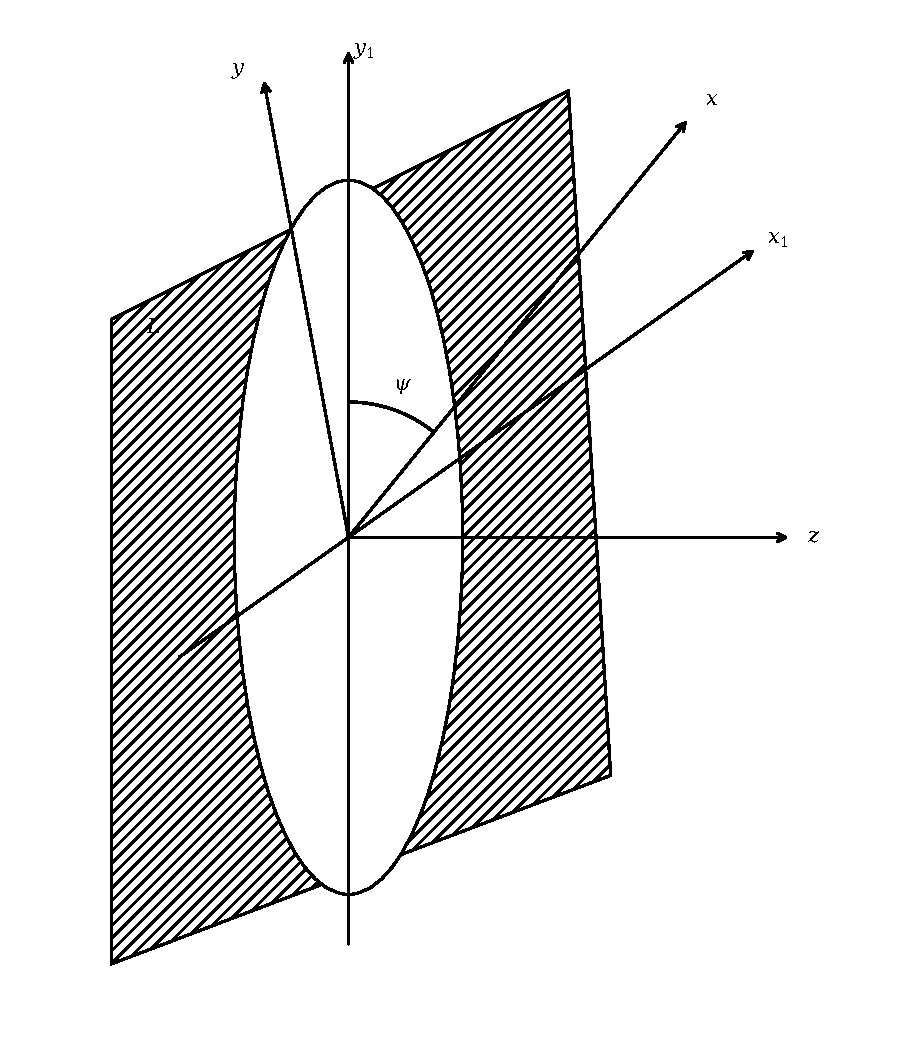
\includegraphics[height=5cm]{images/recreated/a-0067-fig19.pdf}\par Figure 19. Diffraction by a disk. The half-plane $L$ lies in the plane of the disk. The edge of the half-plane is tangent to the circumference of the disk at the point $y_1=a$, $x_1=0$ ($a$ is the radius of the disk).\end{minipage}\hfill\begin{minipage}[t]{.53\linewidth}\vspace{0pt}
\[\left.\begin{gathered}\int_{-\infty}^a j_{x_1}^1(\eta)e^{-ik\eta_1\sin\theta}\,d\eta=\\=-\frac{ic}{2\pi k}E_{0x_1}f^1(1)e^{-ika\sin\theta},\\\int_{-\infty}^a j_{x_1}^1(\eta)e^{ik\eta_1\sin\theta}\,d\eta=\\=-\frac{ic}{2\pi k}E_{0x_1}f^1(2)e^{ika\sin\theta}\end{gathered}\right\}\tag{8.09}\]
and
\[\left.\begin{gathered}\int_{-\infty}^a j_{y_1}^1(\eta)e^{-ik\eta_1\sin\theta}\,d\eta=\\=\frac{ic}{2\pi k\cos\theta}H_{0x_1}g^1(1)e^{-ika\sin\theta},\\\int_{-\infty}^a j_{y_1}^1(\eta)e^{ik\eta_1\sin\theta}\,d\eta=\\=\frac{ic}{2\pi k\cos\theta}H_{0x_1}g^1(2)e^{ika\sin\theta}.\end{gathered}\right\}\tag{8.10}\]
\end{minipage}
In accordance with the assumption of equal currents on the disk and on the half-plane, one may consider the following equalities to be valid:
\[\left.\begin{aligned}\int_0^a\mathbf j^1(\rho,\psi_1)e^{-ik\rho\sin\theta}\,d\rho&=\int_{-\infty}^a\mathbf j^1(\eta)e^{-ik\eta_1\sin\theta}\,d\eta,\\\int_0^a\mathbf j^1(\rho,\psi_2)e^{ik\rho\sin\theta}\,d\rho&=\int_{-\infty}^a\mathbf j^1(\eta)e^{ik\eta_1\sin\theta}\,d\eta.\end{aligned}\right\}\tag{8.11}\]
Therefore, the field from the nonuniform part of the current flowing on the disk will equal
\[\left.\begin{aligned}E_\phi=-H_\theta&=\frac{iaE_{0\phi}}{\sqrt{2\pi ka\sin\theta}}\left[f^1(2)e^{i(ka\sin\theta-\frac{3\pi}4)}-\right.\\&\qquad\left.-f^1(1)e^{-i(ka\sin\theta-\frac{3\pi}4)}\right]\frac{e^{ikR}}R,\\E_\theta=H_\phi&=\frac{iaH_{0\phi}}{\sqrt{2\pi ka\sin\theta}}\left[g^1(2)e^{i(ka\sin\theta-\frac{3\pi}4)}-\right.\\&\qquad\left.-g^1(1)e^{-i(ka\sin\theta-\frac{3\pi}4)}\right]\frac{e^{ikR}}R,\end{aligned}\right\}\tag{8.12}\]
where in view of (7.01)
\[E_{0\phi}=-H_{0x}\cos\phi,\quad H_{0\phi}=-H_{0x}\sin\phi.\tag{8.13}\]
\endgroup
\end{scanpage}
